%%% PREAMBLE - Do not touch %%%%%%%%%%%%%%%%%%%%%%%%%%%%%%%%%%%%%%%%%%%%%%%%%%%%%%
\documentclass[10pt,twocolumn,letterpaper]{article}
\usepackage[utf8]{inputenc}
\usepackage[T1]{fontenc}
\usepackage[portuges,brazilian,english]{babel}
\usepackage{model}
\usepackage{times}
\usepackage{epsfig}
\usepackage{graphicx}
\usepackage{amsmath}
\usepackage{amssymb}
\usepackage{color}
\usepackage[pagebackref=true,breaklinks=true,letterpaper=true,colorlinks,bookmarks=false]{hyperref}
%  ABACO -- Conjunto de macros para desenhar o 'abaco
%  Desenho original de Hans Liesenberg
%  Macros de Tomasz Kowaltowski
%  DCC -- IMECC -- UNICAMP
%  Mar,co de 1988  --  Vers~ao 1.0
% Ajustado para LaTeX da SUN -- Mar,co de 1991
% ---------------------------------------------------------
%  Chamada:   \ABACO{d1}{d2}{d3}{d4}{esc}
%             com:  di's -- os quatro d'igitos;
%                   esc  -- fator de escala
% ---------------------------------------------------------
%  DEFINI,C~OES AUXILIARES
% ---------------------------------------------------------
%  Forma o d'igito pequeno (0 ou 1)

\newcommand{\ABACODP}[1]{%
%
\thicklines
%    
\begin{picture}(8,0)
    \ifcase#1{   %  caso 0
       \put(0,0)    {\line(1,0){4}}
       \multiput(5,0)(2,0){2}{\oval(2,4)}}
    \or{         %  caso 1
       \put(2,0)    {\line(1,0){4}}
       \multiput(1,0)(6,0){2}{\oval(2,4)}}
    \fi
\end{picture}
    } % \ABACODP

% Forma o d'igito grande (0 a 4)

\newcommand{\ABACODG}[1]{%
%
\thicklines
%    
\begin{picture}(14,0)
    \ifcase#1{   % caso 0
       \multiput(1,0)(2,0){5}{\oval(2,4)}}
       \put(10,0)   {\line(1,0){4}}
    \or{         % caso 1
       \multiput(1,0)(2,0){4}{\oval(2,4)}}
       \put(8,0)   {\line(1,0){4}}
       \put(13,0)   {\oval(2,4)}
    \or{         % caso 2
       \multiput(1,0)(2,0){3}{\oval(2,4)}
       \put(6,0)   {\line(1,0){4}}
       \multiput(11,0)(2,0){2}{\oval(2,4)}}
    \or{         % caso 3
       \multiput(1,0)(2,0){2}{\oval(2,4)}
       \put(4,0)   {\line(1,0){4}}
       \multiput(9,0)(2,0){3}{\oval(2,4)}}
    \or{         % caso 4
       \put(1,0)  {\oval(2,4)}}
       \put(2,0)   {\line(1,0){4}}
       \multiput(7,0)(2,0){4}{\oval(2,4)}
    \fi
\end{picture}
    } % \ABACODG
       
% Forma um d'igito (0 a 9)

\newcommand{\ABACOD}[1]{%
%
    \ifnum#1>9
       \errmessage{#1: Argumento invalido para ABACO}
    \fi
    \ifnum#1<0
       \errmessage{#1: Argumento invalido para ABACO}
    \fi
%
\begin{picture}(24,0)
%    
    \ifnum#1<5
       \put(16,0) {\ABACODP{0}}
    \else   
       \put(16,0) {\ABACODP{1}}
    \fi
%    
    \ifnum#1<5
       \put(0,0)  {\ABACODG{#1}}
    \else
       \ifcase#1\or \or \or \or
          \or  \put(0,0)  {\ABACODG{0}}
          \or  \put(0,0)  {\ABACODG{1}}
          \or  \put(0,0)  {\ABACODG{2}}
          \or  \put(0,0)  {\ABACODG{3}}
          \or  \put(0,0)  {\ABACODG{4}}
       \fi
    \fi   
\end{picture}
    } % \ABACOD
    
% -------------------------------------------------

%  DEFINI,C~AO PRINCIPAL
    
\newcommand{\ABACO}[5]{%
    \setlength{\unitlength}{#5mm}
%
    \thinlines
%   
\begin{picture}(28,25)
%   
% moldura
%
% externa
%
        \put(0,0)            {\line(0,1){25}}
        \put(0,0)            {\line(1,0){28}}
        \put(28,0)           {\line(0,1){25}}
        \put(0,25)           {\line(1,0){28}}
% interna
        \put(2,2)            {\line(0,1){21}}
        \put(26,2)           {\line(0,1){21}}
        \put(16,2)           {\line(0,1){21}}
        \put(18,2)           {\line(0,1){21}}
        \put(2,2)            {\line(1,0){14}}
%        \put(16,2)           {\line(1,-1){1}}
%        \put(17,1)           {\line(1,1){1}}
        \put(18,2)           {\line(1,0){8}}
        \put(2,23)           {\line(1,0){14}}
%        \put(16,23)          {\line(1,1){1}}
%       \put(17,24)          {\line(1,-1){1}}
        \put(18,23)          {\line(1,0){8}}
%        \put(0,0)            {\line(1,1){2}}
%        \put(0,25)           {\line(1,-1){2}}
%        \put(28,0)           {\line(-1,1){2}}
%        \put(28,25)          {\line(-1,-1){2}}
%
%   
% d'igitos
%
%   
       \put(2,20)  {\ABACOD{#1}}
       \put(2,15)  {\ABACOD{#2}}
       \put(2,10)  {\ABACOD{#3}}
       \put(2,5)   {\ABACOD{#4}}
%      
\end{picture}
    } % \ABACO
    


\cvprfinalcopy % *** Uncomment this line for the final submission
\def\httilde{\mbox{\tt\raisebox{-.5ex}{\symbol{126}}}}
\ifcvprfinal\pagestyle{empty}\fi

\newcommand{\TODO}[1]{TODO: #1}
\newcommand{\CITEONE}[2]{\mbox{#1 \cite{#2}}}
\newcommand{\CITETWO}[3]{\mbox{#1 and #2 \cite{#3}}}
\newcommand{\CITEN}[2]{\mbox{#1 et al. \cite{#2}}}

%%% Report beginning %%%%%%%%%%%%%%%%%%%%%%%%%%%%%%%%%%%%%%%%%%%%%%%%%%%%%%%%%%%%%%
\begin{document}

%%% Title and authors %%%%%%%%%%%%%%%%%%%%%%%%%%%%%%%%%%%%%%%%%%%%%%%%%%%%%%%%%%%%
\title{Image Panorama Stitching}
\author{Thalles Santos Silva\thanks{Is with the Institute of Computing, University of Campinas (Unicamp). \textbf{Contact}: \tt\small{thalles753@gmail.com}}\\
Hélio Pedrini\thanks{Is with the Institute of Computing, University of Campinas (Unicamp). \textbf{Contact}: \tt\small{helio@ic.unicamp.br}}
}

%%% Abstract %%%%%%%%%%%%%%%%%%%%%%%%%%%%%%%%%%%%%%%%%%%%%%%%%%%%%%%%%%%%%%%%%%%%%
\maketitle
\section{Introduction}

This piece presents a method to perform image stitching using Python and OpenCV. Given a pair of images that share some common region, our goal is to “stitch” them to create panoramic images. 

Our method uses compute vision techniques such as keypoint detection, local invariant descriptors, keypoint matching, hoography estimation using RANSAC and perspective warping. Moreover, we explore many feature extractor algorithms like SIFT, SURF and ORB.

%%% Introduction %%%%%%%%%%%%%%%%%%%%%%%%%%%%%%%%%%%%%%%%%%%%%%%%%%%%%%%%%%%%%%%%%
\section{Setup}

This project was developed using Python version 3 and Jupyter Notebooks. The libraries used across the project are NumPy \cite{NumPy} and OpenCV \cite{OpenCV} to do image-based computation and matplotlib \cite{Matplotlib} for visualization. The Notebook is divided into subsections analogous to the sessions contained in this document.

\section{Feature Detection and Extraction}

Given a pair of images like in Figure \ref{fig:input-images}, the first step to stitch them in a panoramic image is to extract some key points and features of interest.

\begin{figure}[h!]
\begin{center}
	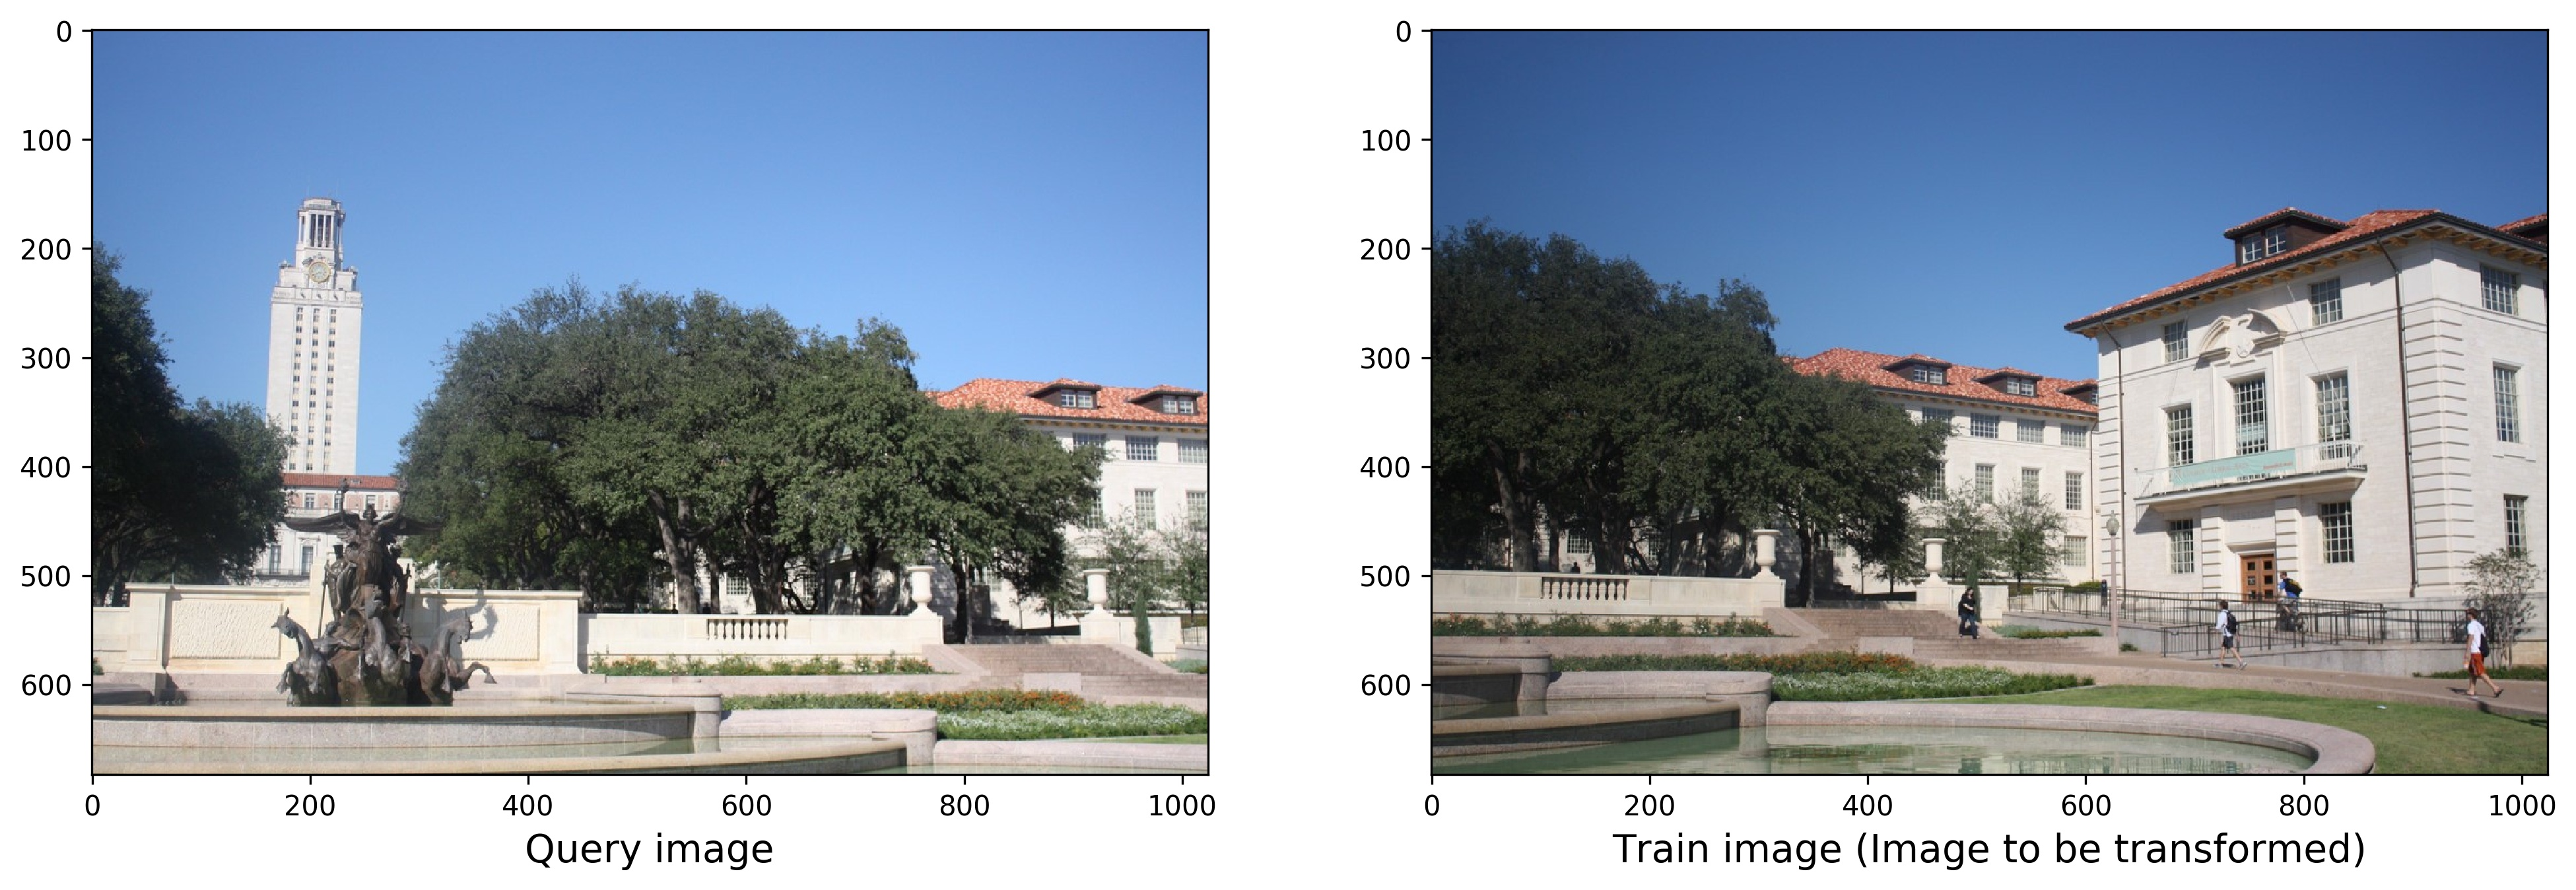
\includegraphics[width=0.99\columnwidth]{pics/input_img_1.jpeg}
	\caption{Input images pair. \label{fig:input-images}}   
\end{center} 
\end{figure}  

These features, however, need to have some special properties. An initial and naive approach would be to extract key points using an algorithm such as Harris Corners. Then, we could try to match the corresponding key points from both images. As we know, corners have one nice property: they are invariant to rotation. In other words, once we detect a corner, if we rotate the image, the corner will still be there.

However, what if we rotate then scale the image? In this situation, we would have a hard time because corners are not invariant to scale. That is to say, if we zoom-in to an image, the previously detected corner might become a line!

In summary, we need features that are invariant to rotation and scaling. That is where more robust methods such as SIFT, SURF, and ORB come in.

In summary, methods like SIFT and SURF try to address the limitations of corner detection algorithms. As we know, corners are not invariant to scale. That is because corner detector algorithms use a fixed size kernel to spot corners on images. It is easy to see that when we scale an image, this kernel might become too small or too big.
To address this limitation, methods like SIFT uses Difference of Gaussians (DoD). The idea is to apply DoD on different scaled versions of the same image. It also uses the neighboring pixel information to find and refine key points and corresponding descriptors.

To start, we need to load 2 images, a query image, and a training image. Initially, we begin by extracting key points and descriptors from both. We can do it in one step by using the OpenCV detectAndCompute() function. Note that in order to use detectAndCompute() we need an instance of a keypoint detector and descriptor object. It can be ORB, SIFT or SURF, etc. Also, before feeding the images to detectAndCompute() we convert it to grayscale.
We run detectAndCompute() on both, the query and the train image. At this point, we have a set of key points and descriptors for both images. If we use SIFT as the feature extractor, it returns a 128 dimensional feature vector for each key point. If SURF is chosen, we get a 64-dimensional feature vector. Figures \ref{fig:sift-features}, \ref{fig:surf-features}, \ref{fig:brisk-features}, and \ref{fig:orb-features} show features extracted using SIFT, SURF, BRISK, and ORB.

\begin{figure}[h!]
\begin{center}
	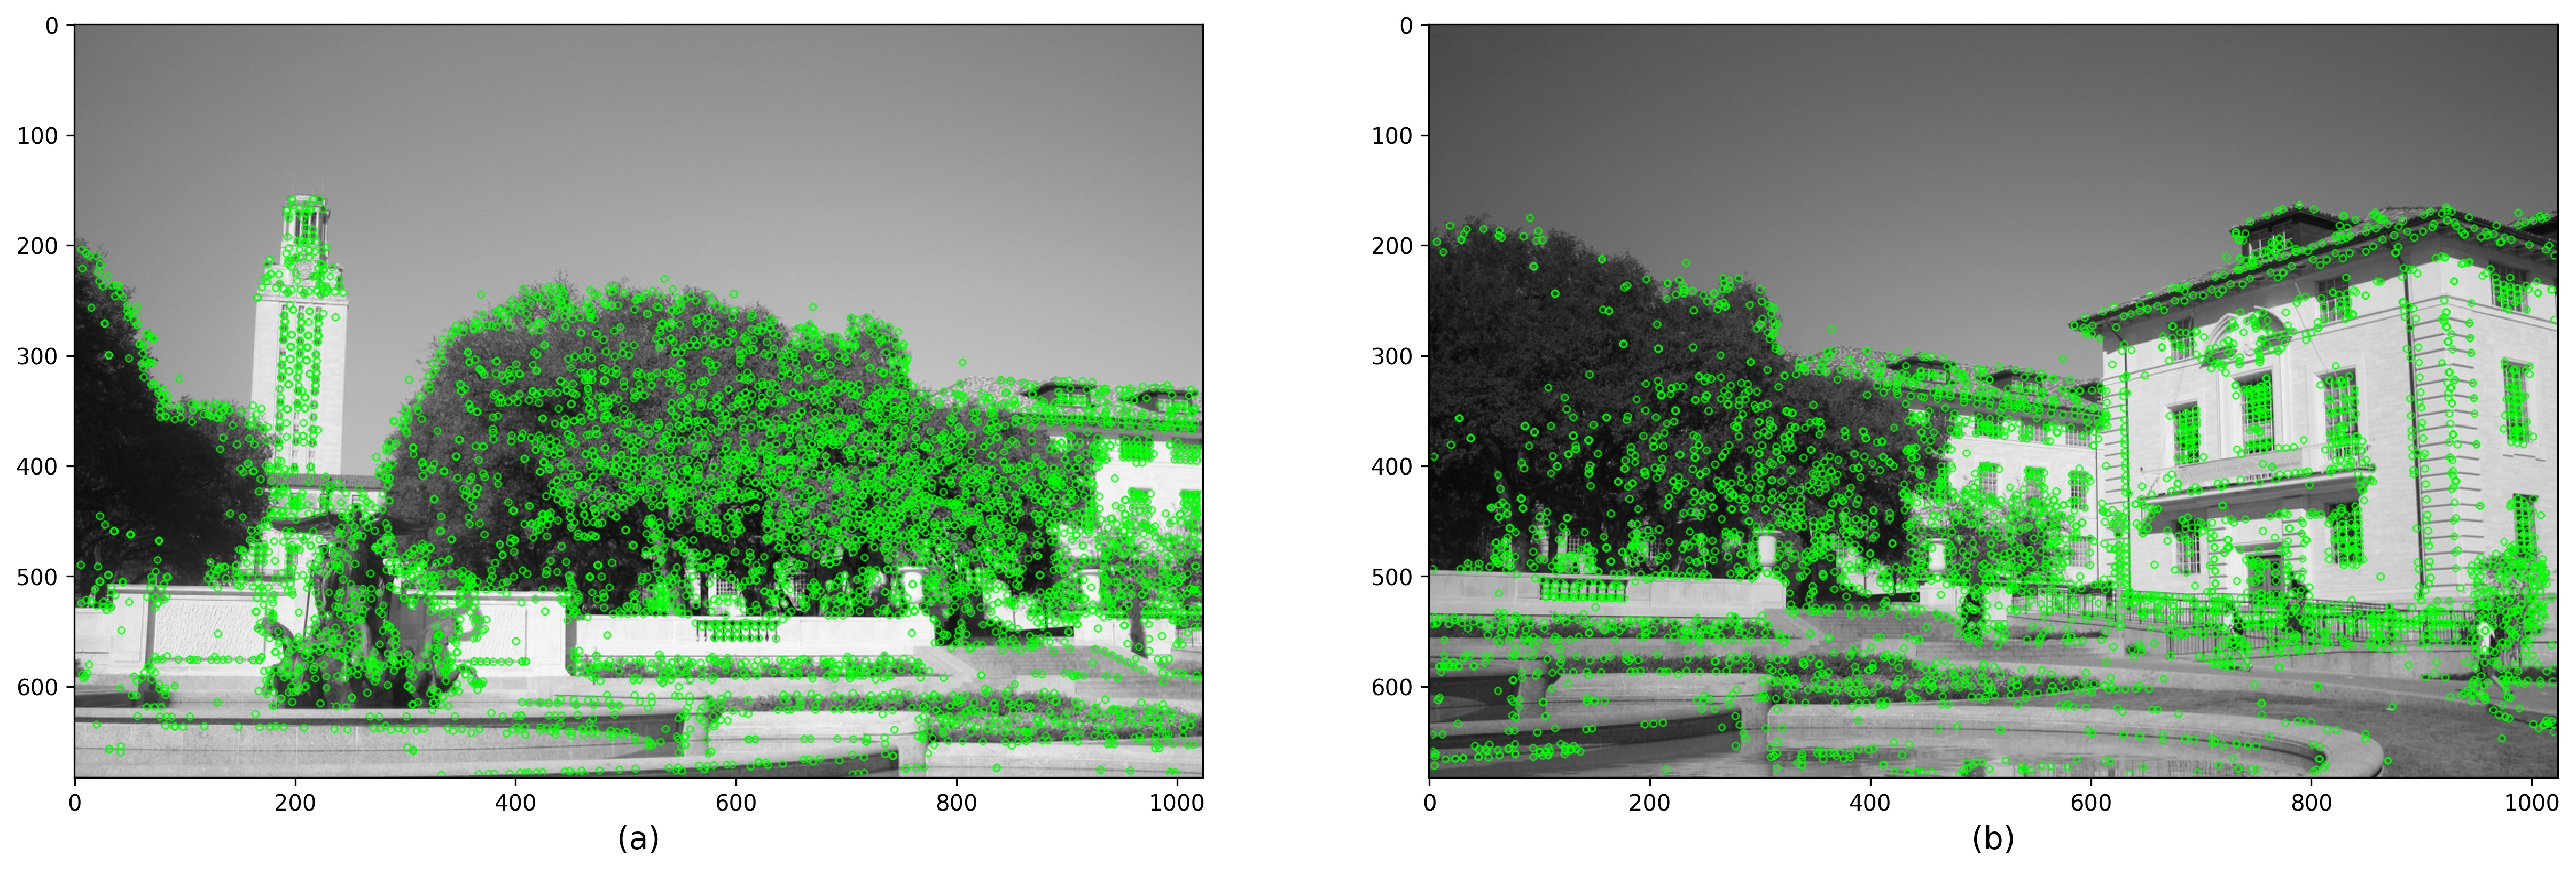
\includegraphics[width=0.99\columnwidth]{pics/sift_features_img_1.jpeg}
	\caption{Detection of key points and descriptors using SIFT. \label{fig:sift-features}}   
\end{center} 
\end{figure}  

\begin{figure}[h!]
\begin{center}
	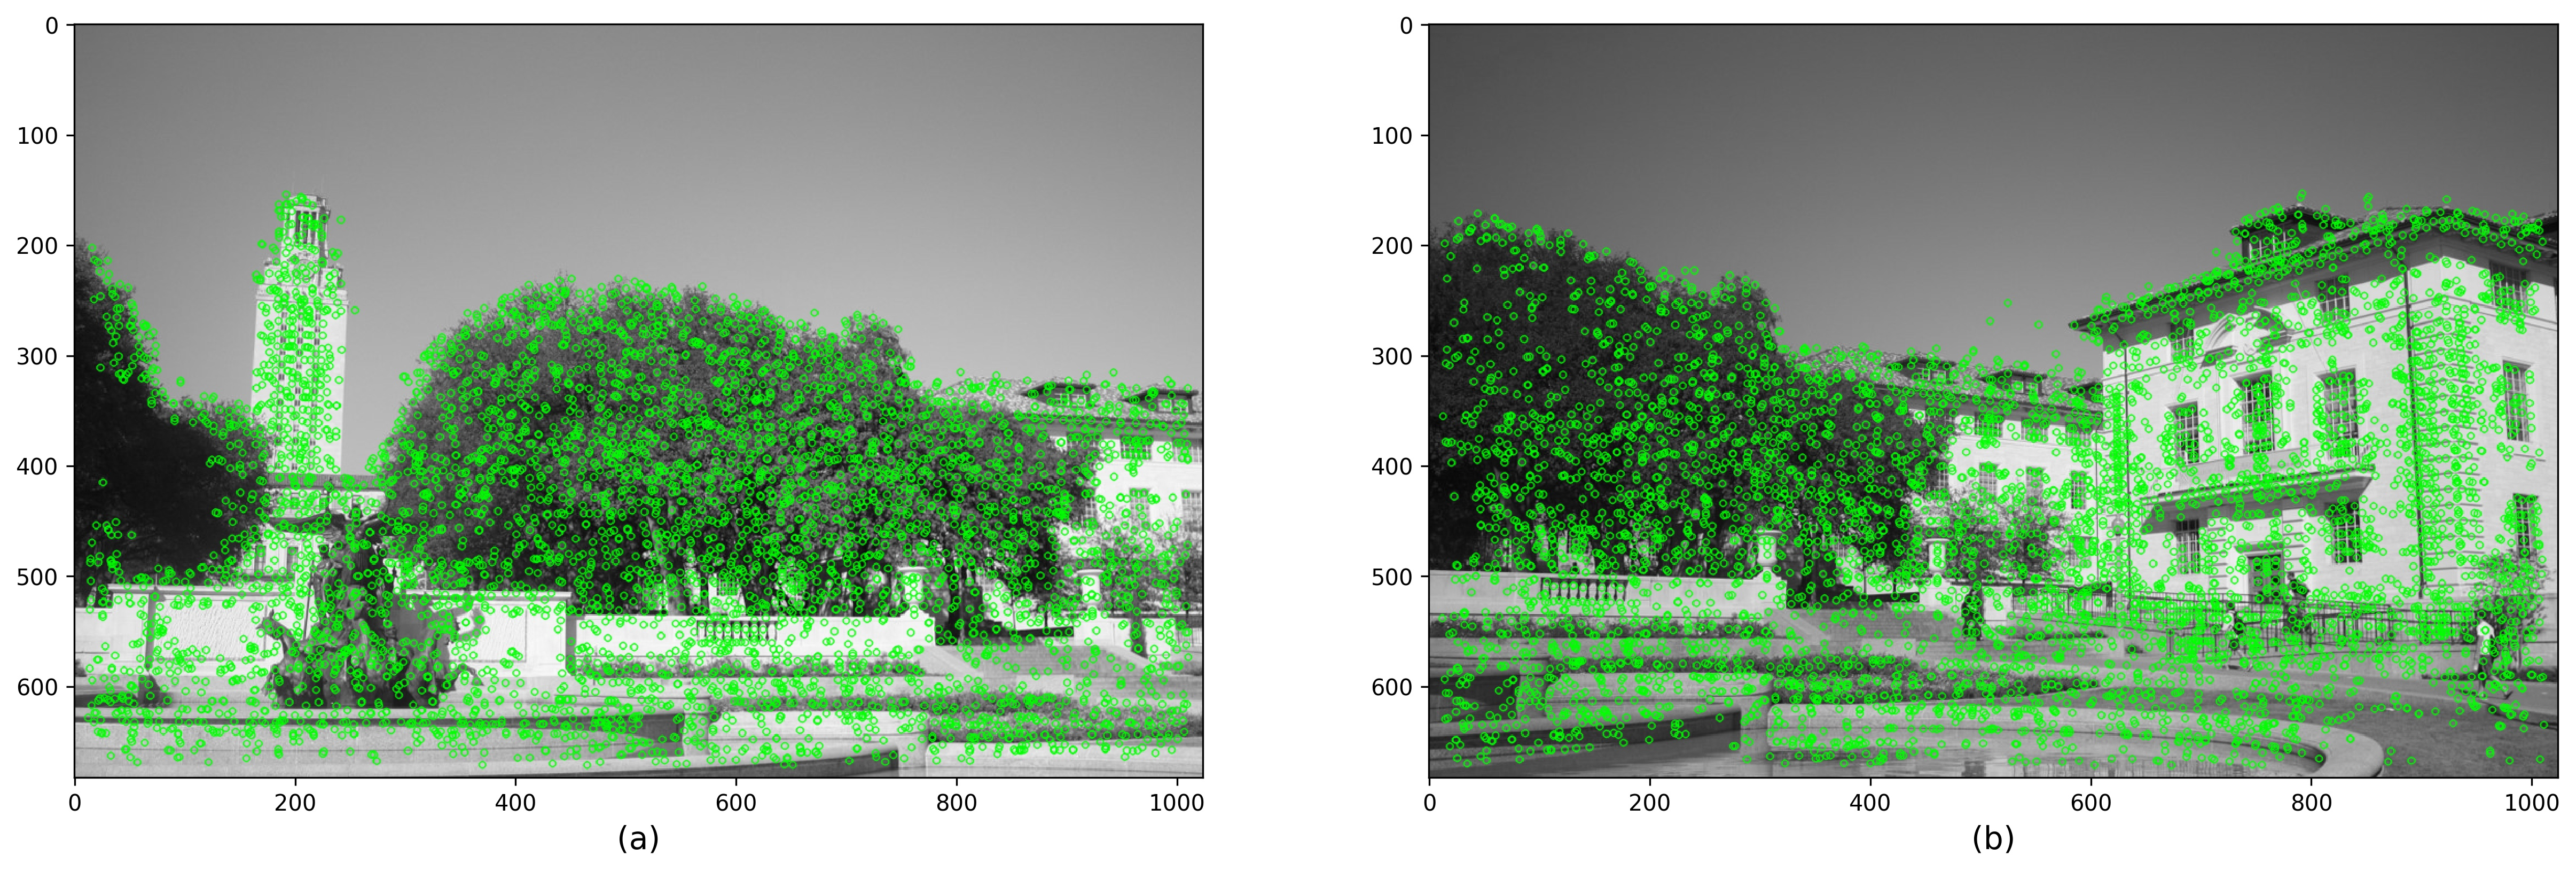
\includegraphics[width=0.99\columnwidth]{pics/surf_features_img_1.jpeg}
	\caption{Detection of key points and descriptors using SURF. \label{fig:surf-features}}   
\end{center} 
\end{figure}  

\begin{figure}[h!]
\begin{center}
	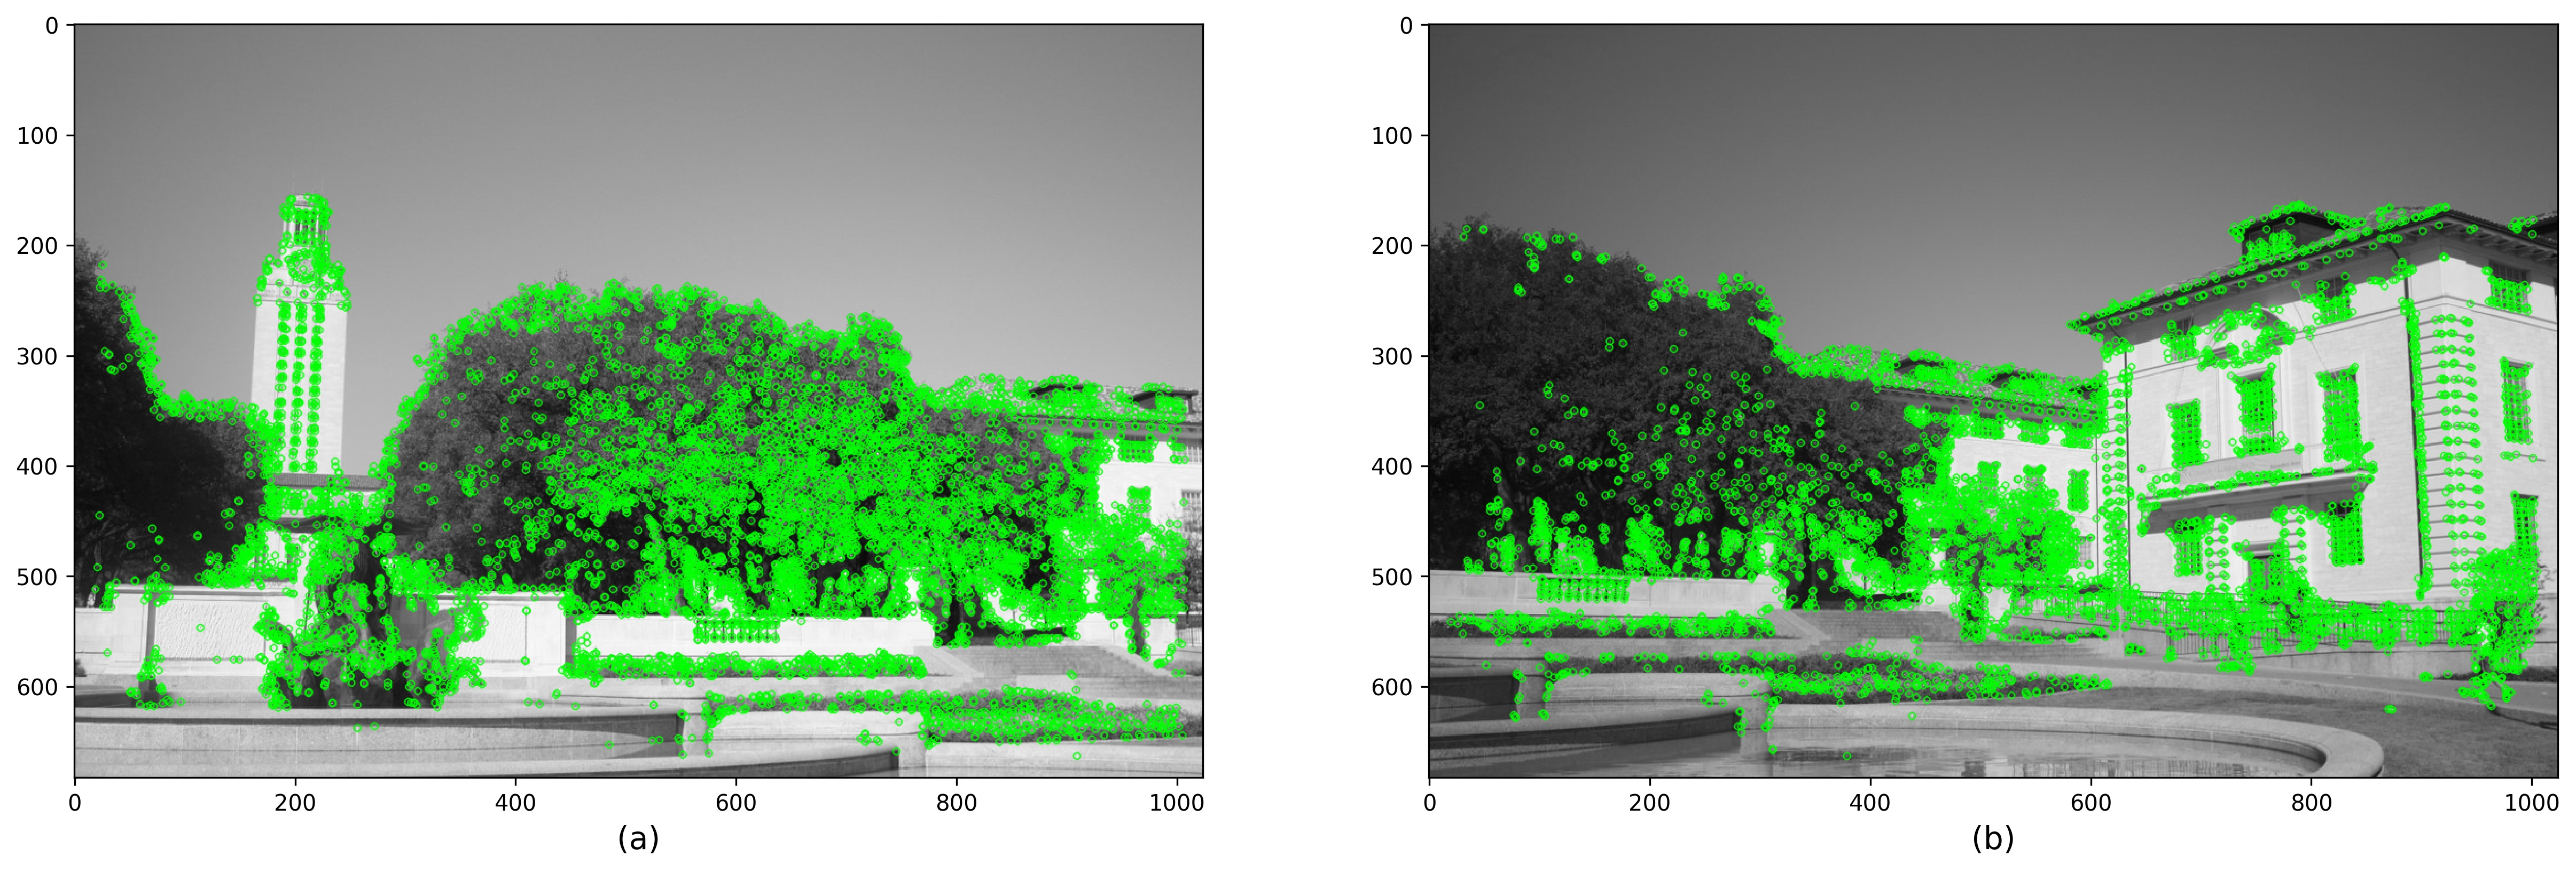
\includegraphics[width=0.99\columnwidth]{pics/brisk_features_img_1.jpeg}
	\caption{Detection of key points and descriptors using BRISK and Hamming distances. \label{fig:brisk-features}}   
\end{center} 
\end{figure}  

\begin{figure}[h!]
\begin{center}
	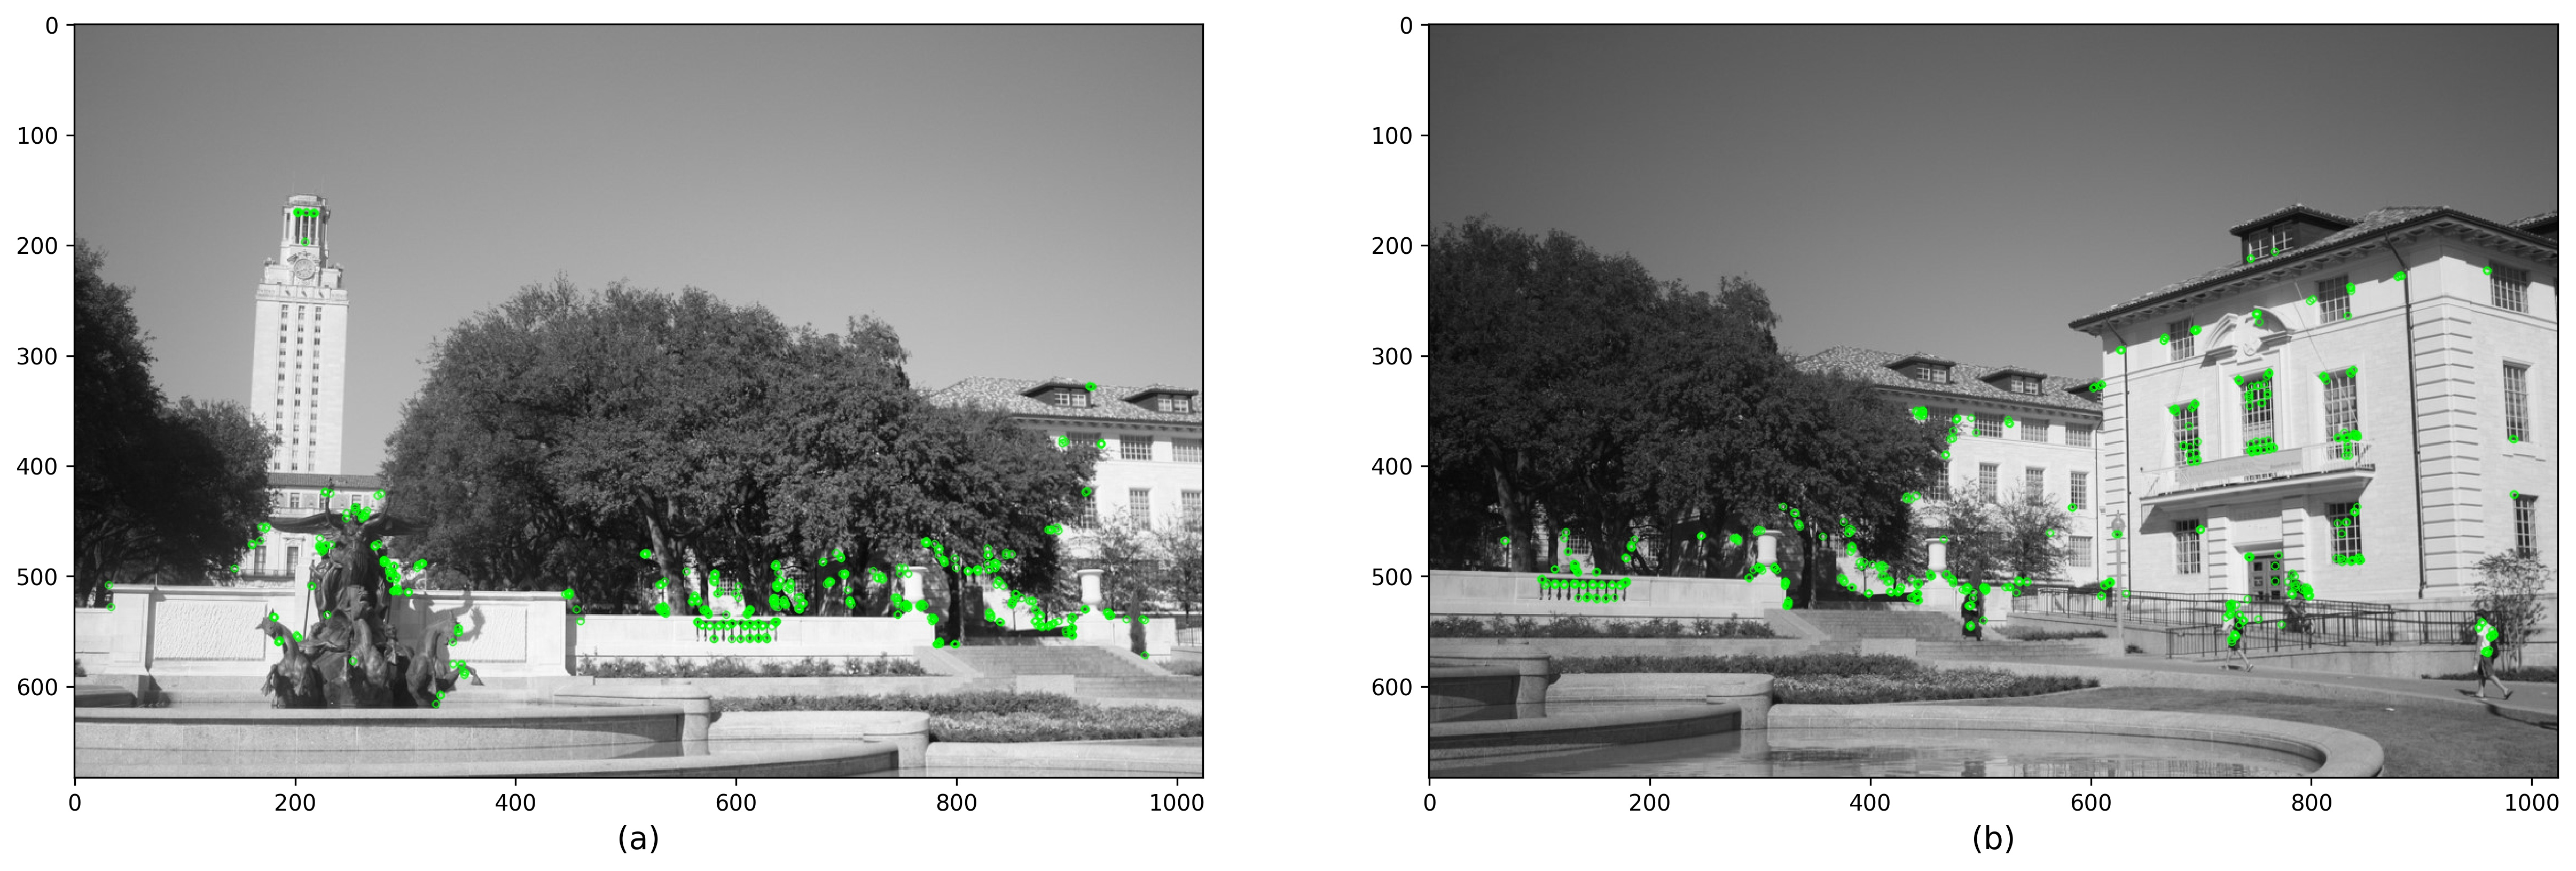
\includegraphics[width=0.99\columnwidth]{pics/orb_features_img_1.jpeg}
	\caption{Detection of key points and descriptors using ORB and Hamming distances. \label{fig:orb-features}}   
\end{center} 
\end{figure}  

\subsection{Feature Matching}

As we can see, we have a large number of features in both images. The next step is to compare the 2 sets of features and stick with the pairs that show more similarity. This process is called feature matching.
With OpenCV, feature matching requires a Matcher object. Here, we explore two flavors: KNN (k-nearest neighbors) and Brute Force.

The BruteForce (BF) Matcher does exactly what its name suggests. Given 2 sets of features (from image A and image B), each feature from image A is compared against all features from image B. By default, BF Matcher computes the Euclidean distance from two points. Thus, for every feature in set A, it returns the closest feature from the set B. For SIFT and SURF OpenCV recommends using Euclidean distance. For other feature extractors like ORB and BRISK, Hamming distance is suggested.

To create a BruteForce Matcher using OpenCV we only need to specify 2 parameters. The first, is the distance measurement. The second, is the crossCheck boolean parameter. It indicates whether the two features have to match each other to be considered valid matches. In other words, for a pair of features (f1, f2) to considered valid, f1 needs to match f2 and f2 has to match f1 as the closest match as well. This procedure ensures a more robust set of matching features and is described in the original SIFT paper.

However, for the case where we want to consider more than one good match, we can use the KNN Matcher. Instead of returning the only best match for a given feature, KNN returns the k best matches. Note that the value of k has to be pre-defined by the user.

As we expect, KNN provides a larger set of candidate features. However, we need to ensure that all these matching pairs are robust before going further.

\subsection{Ratio Testing}

D. Lowe, the author of the SIFT paper, suggests a technique called ratio test. Basically, we iterate over each of the pairs returned by KNN and perform a distance test. For each pair of features (f1, f2), if the distance between f1 and f2 is within a certain ratio, we keep it, otherwise, we through it away. Also, the ratio value must be chosen manually.

In essence, the ratio test does the same job as the cross-checking procedure from the BruteForce Matcher. Both, ensure a pair of detected features are indeed close enough to be considered similar. Figures \ref{fig:bf-matching} and \ref{fig:knn-matching} show the results of BF and KNN Matcher on the SIFT features. We chose to displays only 100 matching points to clear understanding.

\begin{figure}
\begin{center}
	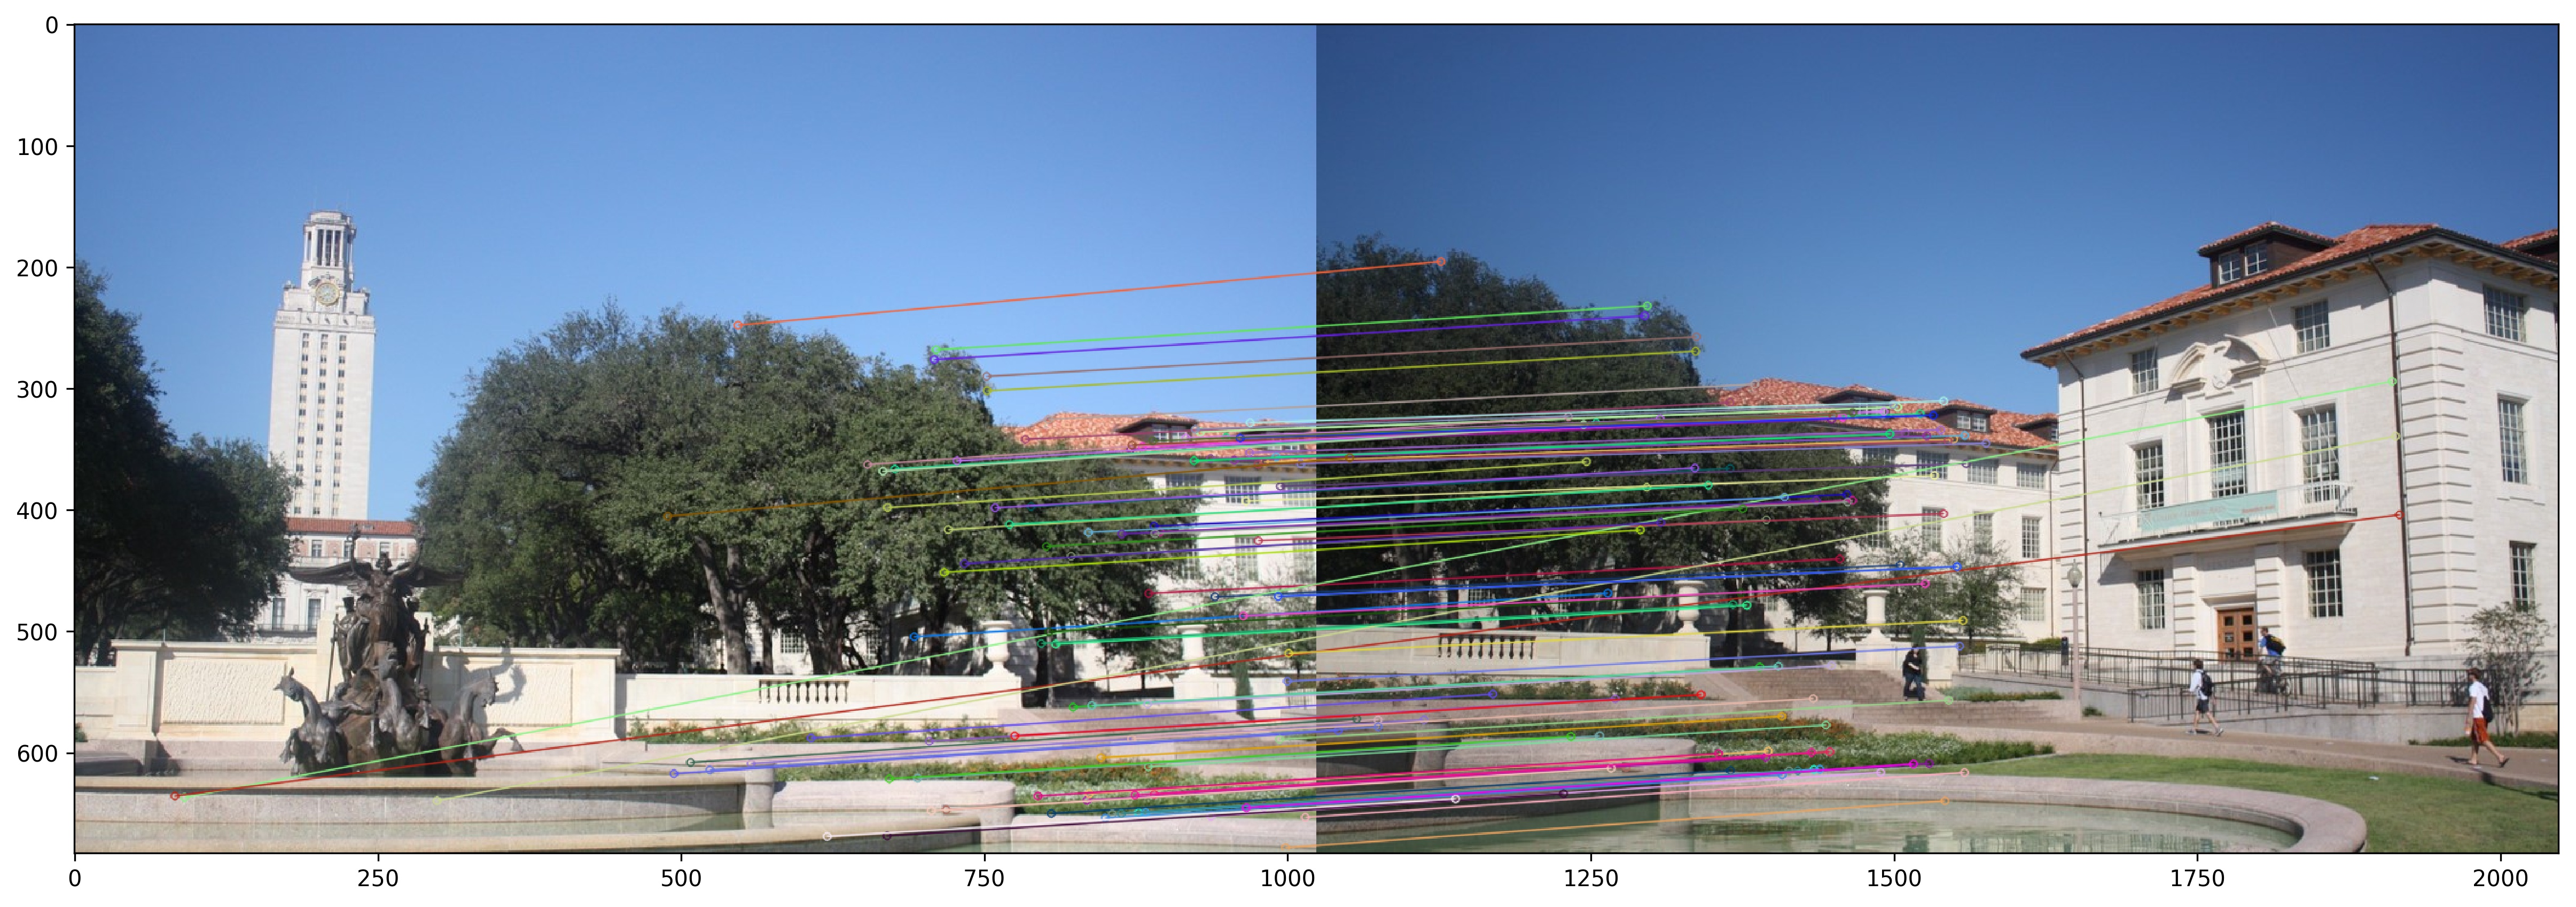
\includegraphics[width=0.99\columnwidth]{pics/bf_matching_img_1.jpeg}
	\caption{Feature matching using Brute Force Matcher on SIFT features. \label{fig:bf-matching}}   
\end{center} 
\end{figure}  

\begin{figure}
\begin{center}
	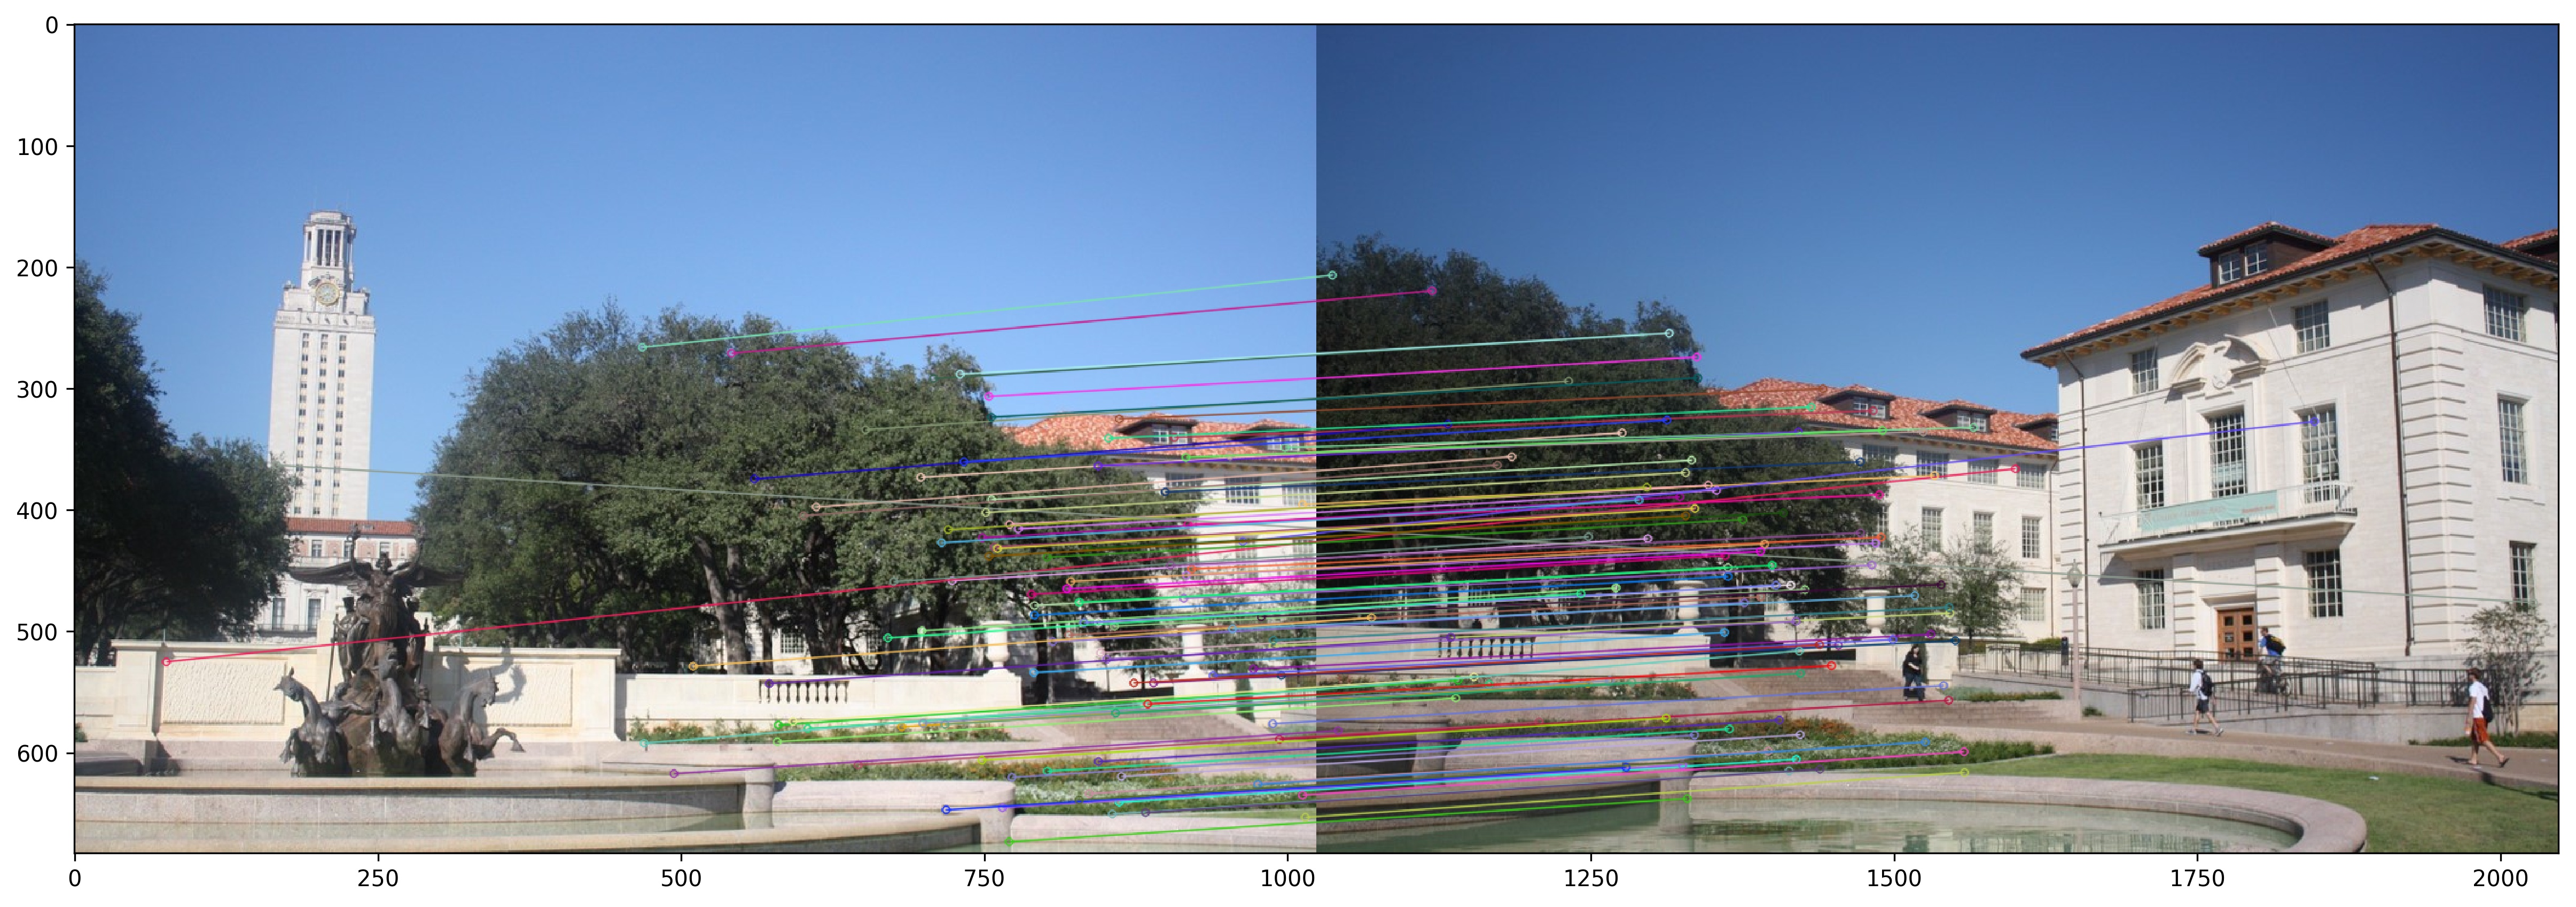
\includegraphics[width=0.99\columnwidth]{pics/knn_matching_img_1.jpeg}
	\caption{Feature matching using KNN and Ration Testing on SIFT features. \label{fig:knn-matching}}   
\end{center} 
\end{figure}

Note that even after cross-checking for Brute force and ratio testing in KNN, some of the features do not match properly.

The Matcher algorithm will give us the best (more similar) set of features from both images. Now, we need to take these points and find the transformation matrix that will stitch the 2 images together based on their matching points.

Such a transformation is called the Homography matrix. In short, it is a 3x3 matrix that can be used in many applications such as camera pose estimation, perspective correction, and image stitching. The Homography is a 2D transformation. It maps points from one plane (image) to another. Let's see how we get it.

\subsection{Estimating the Homography}

RANdom SAmple Consensus or RANSAC is an iterative algorithm to fit linear models. Different from other linear regressors, RANSAC is designed to be robust to outliers. Basically, models like Linear Regression uses least squares estimation to fit the best model to the data. However, ordinary least squares is very sensitive to outliers. As a result, it might fail if the number of outliers is significant.

As an answer, RANSAC solves this problem by estimating parameters only using a subset of inliers in the data. Figure \ref{fig:ransac-fitting} shows a comparison between Linear Regression and RANSAC. First, note that the dataset in Figure \ref{fig:ransac-fitting} contains a fairly high number of outliers.

We can see that the Linear Regression model gets easily influenced by the outliers. That is because it is trying to reduce the average error. Thus, it tends to favor models that minimize the overall distance from all data points to the model itself. That includes the outliers.

On the contrary, RANSAC only fits the model on the subset of points identified as the inliers.
This characteristic is very important to our use case. For panorama stitching, we are going to use RANSAC to estimate the Homography matrix. It turns out that the Homography is very sensitive to the quality of data we pass to it. Hence, it is important to have an algorithm (RANSAC) that can separate inliers from outliers.

\begin{figure}[h!]
\begin{center}
	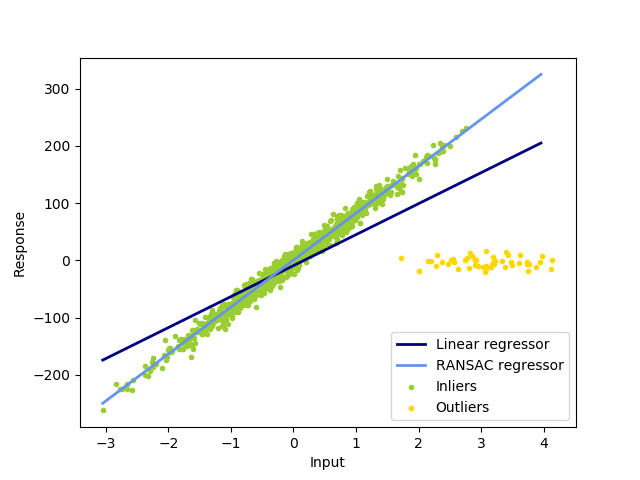
\includegraphics[width=0.80\columnwidth]{pics/ransac.png}
	\caption{RANSAC model fitting.\label{fig:ransac-fitting}}   
\end{center} 
\end{figure} 

To estimate the homography using RANSAC we can use OpenCV findHomography() function. It takes in, the keypoints from the query and train images, and the a reprojection threshold. This threshold defines the maximum allowed reprojection error to treat a point pair as an inlier. For our experiments, the default value of 3.0 worked fine. Figure \ref{fig:ransac-homography} shows an example of an estimated homography matrix using RANSAC.

\begin{figure}[h!]
\begin{center}
	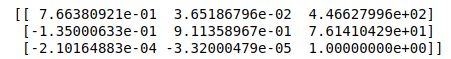
\includegraphics[width=0.80\columnwidth]{pics/homography.png}
	\caption{Homography matrix estimation using RANSAC.\label{fig:ransac-homography}}   
\end{center} 
\end{figure} 

Once we have the Homography between the 2 images estimated (using RANSAC) we need to warp one of the images to a common plane.

Here, we are going to apply a perspective transformation to one of the images. Basically, a perspective transform may combine one or more operations like rotation, scale, translation, or shear. The idea is to transform one of the images so that both images merge as one. To do this, we can use the OpenCV warpPerspective() function. It takes an image and the homography as input. Then, it warps the source image to the destination based on the homography.

Some resulting panoramas are shown in Figures \ref{fig:pan-img-1}, \ref{fig:pan-img-2}, \ref{fig:pan-img-3} and \ref{fig:pan-img-4}. As we see, there are a couple of artifacts in the result. More specifically, we can see some problems related to lighting conditions and edge effects at the image boundaries. Ideally, we can perform post-processing techniques to normalize the intensities like histogram matching. These would likely make the result look more realistic.

\begin{figure*}
\begin{center}
	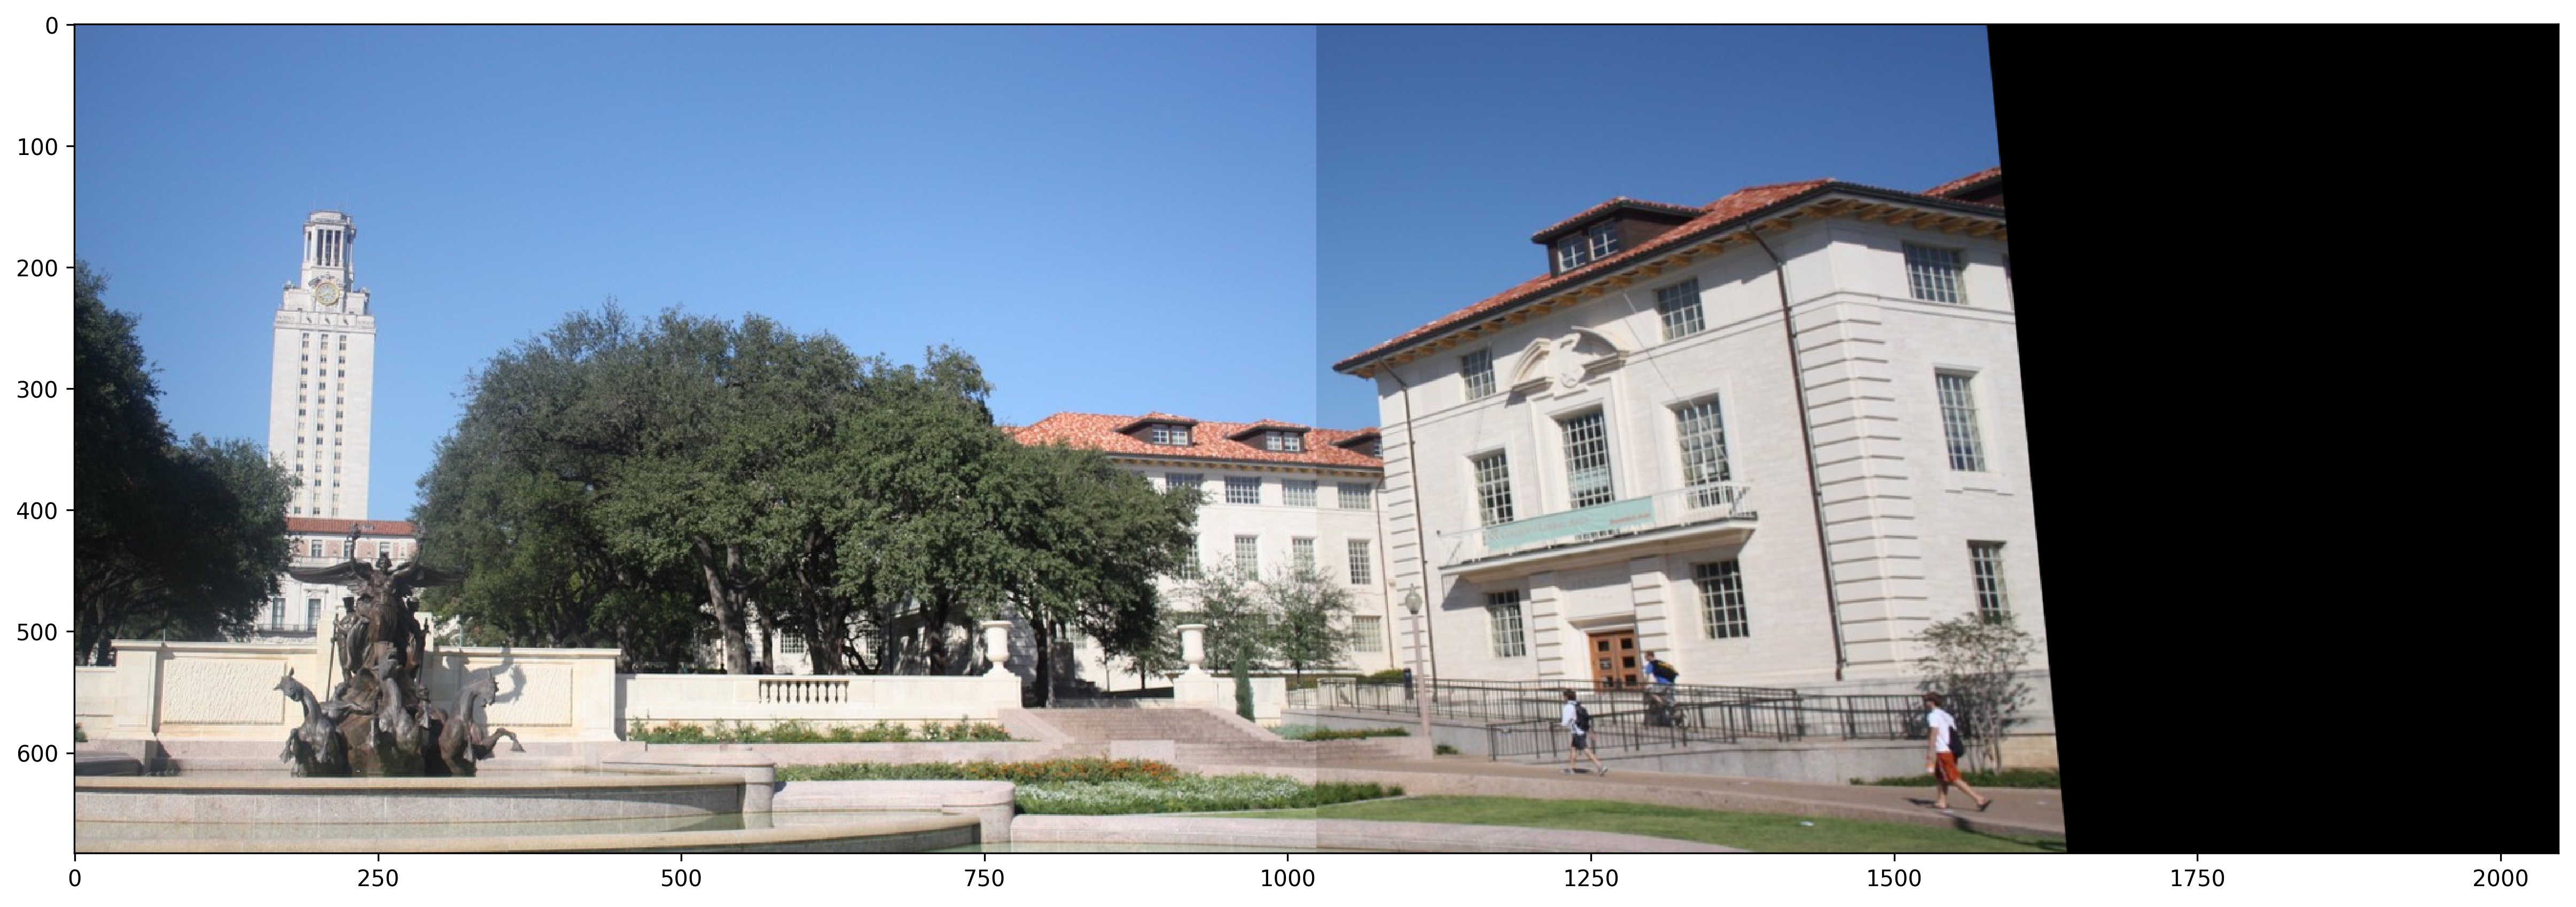
\includegraphics[width=0.99\textwidth]{pics/horizontal_panorama_img_1}
	\caption{. \label{fig:pan-img-1}}   
\end{center} 
\end{figure*}

\begin{figure*}
\begin{center}
	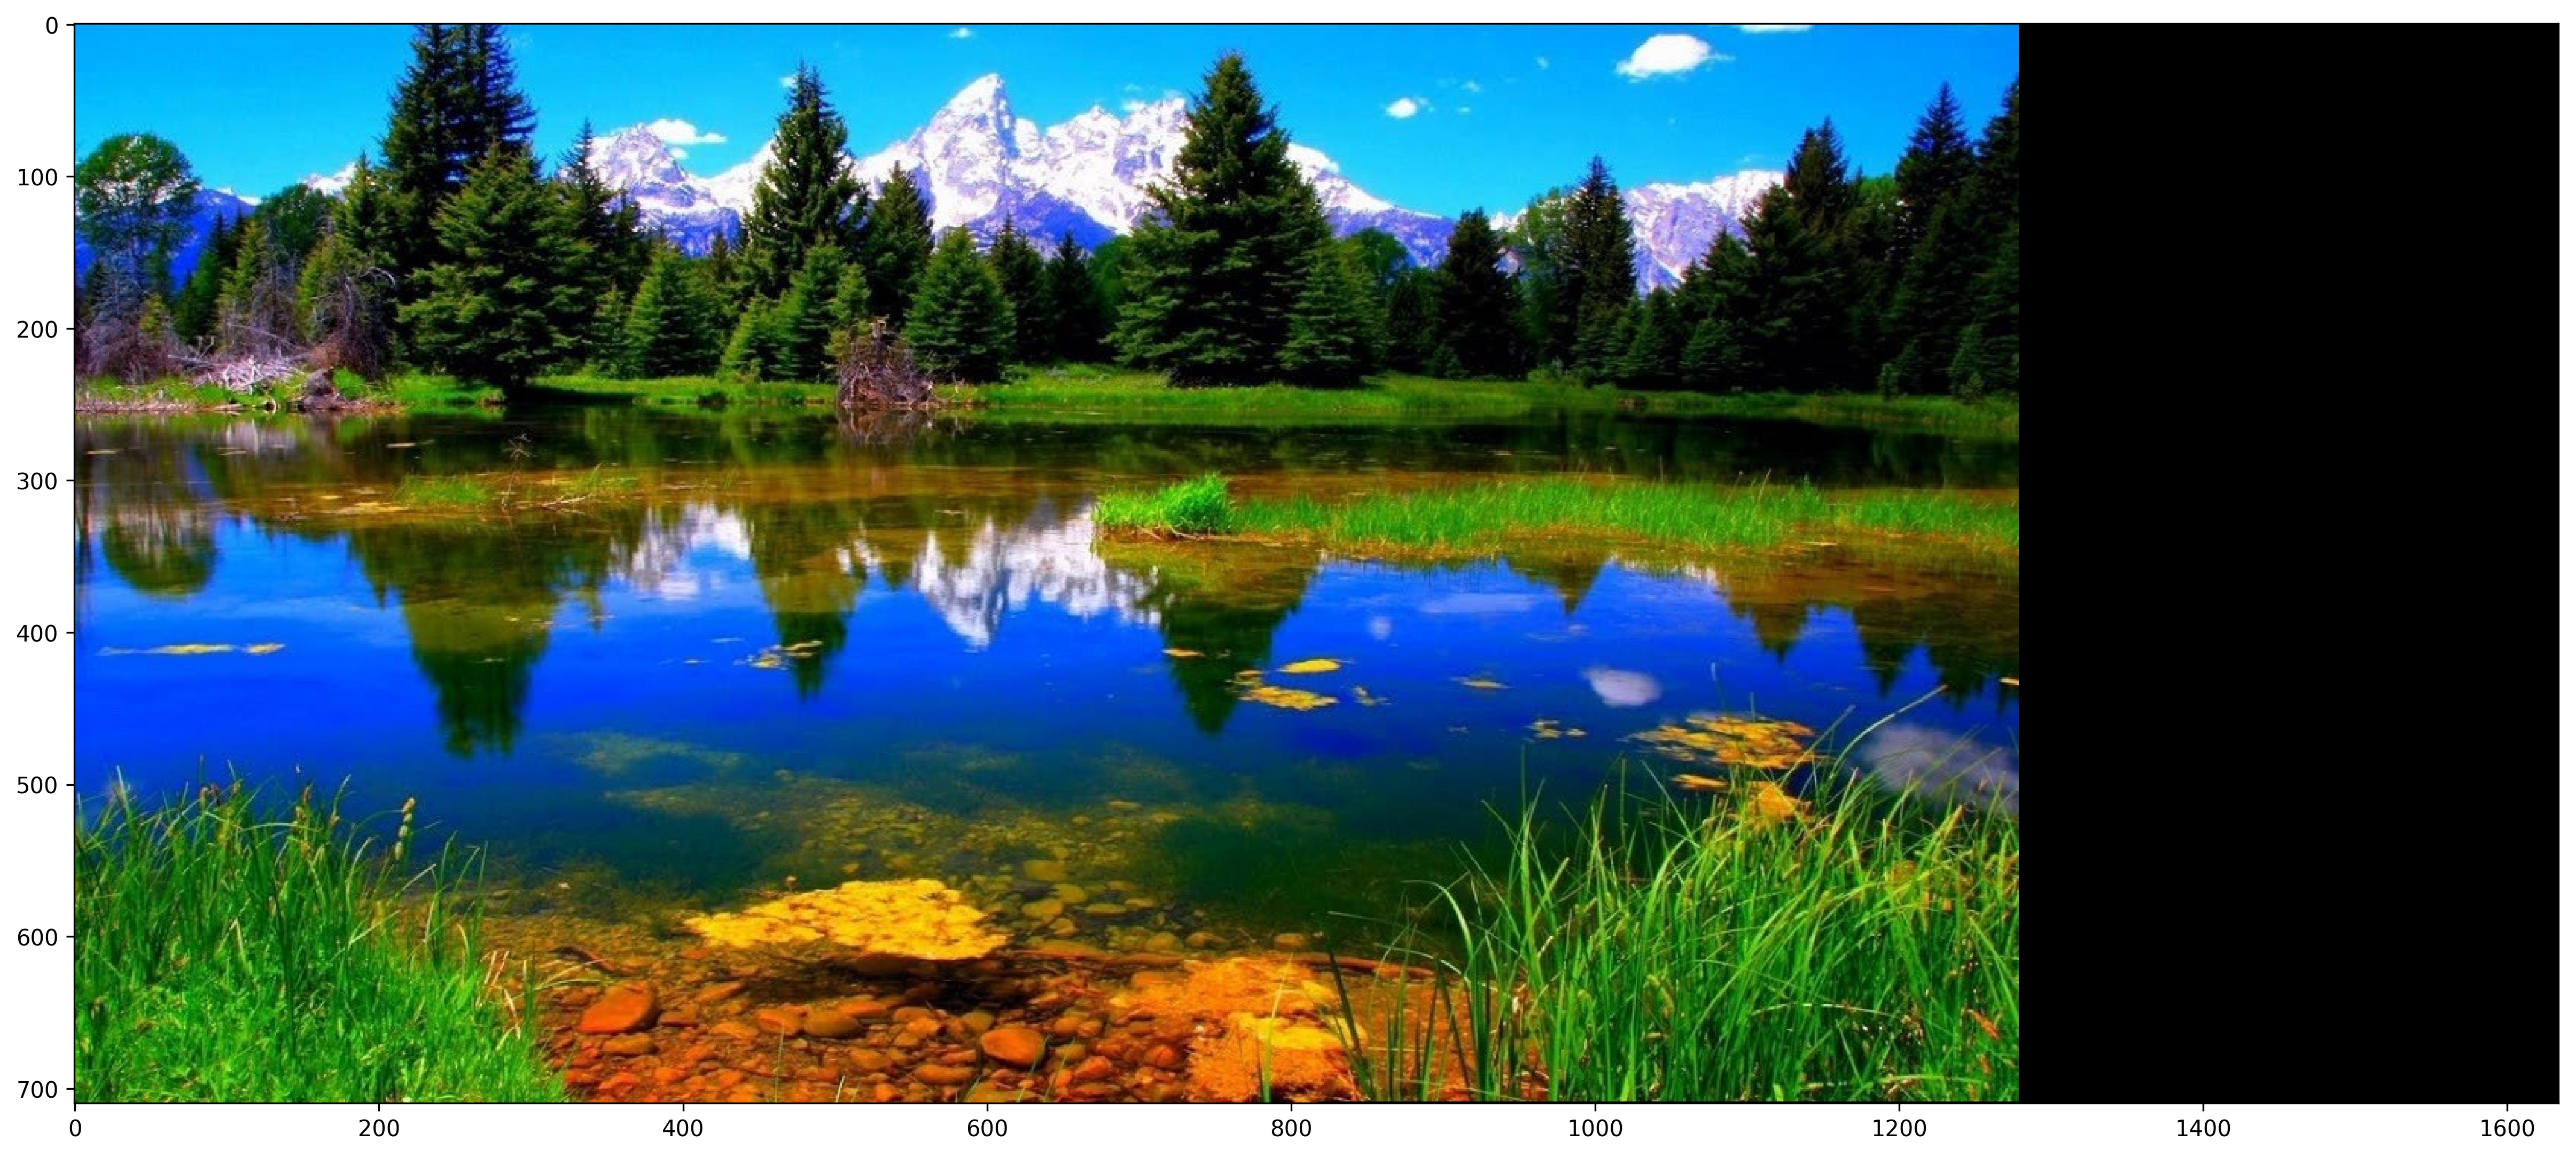
\includegraphics[width=0.99\textwidth]{pics/horizontal_panorama_img_2}
	\caption{. \label{fig:pan-img-2}}   
\end{center} 
\end{figure*}

\begin{figure}
\begin{center}
	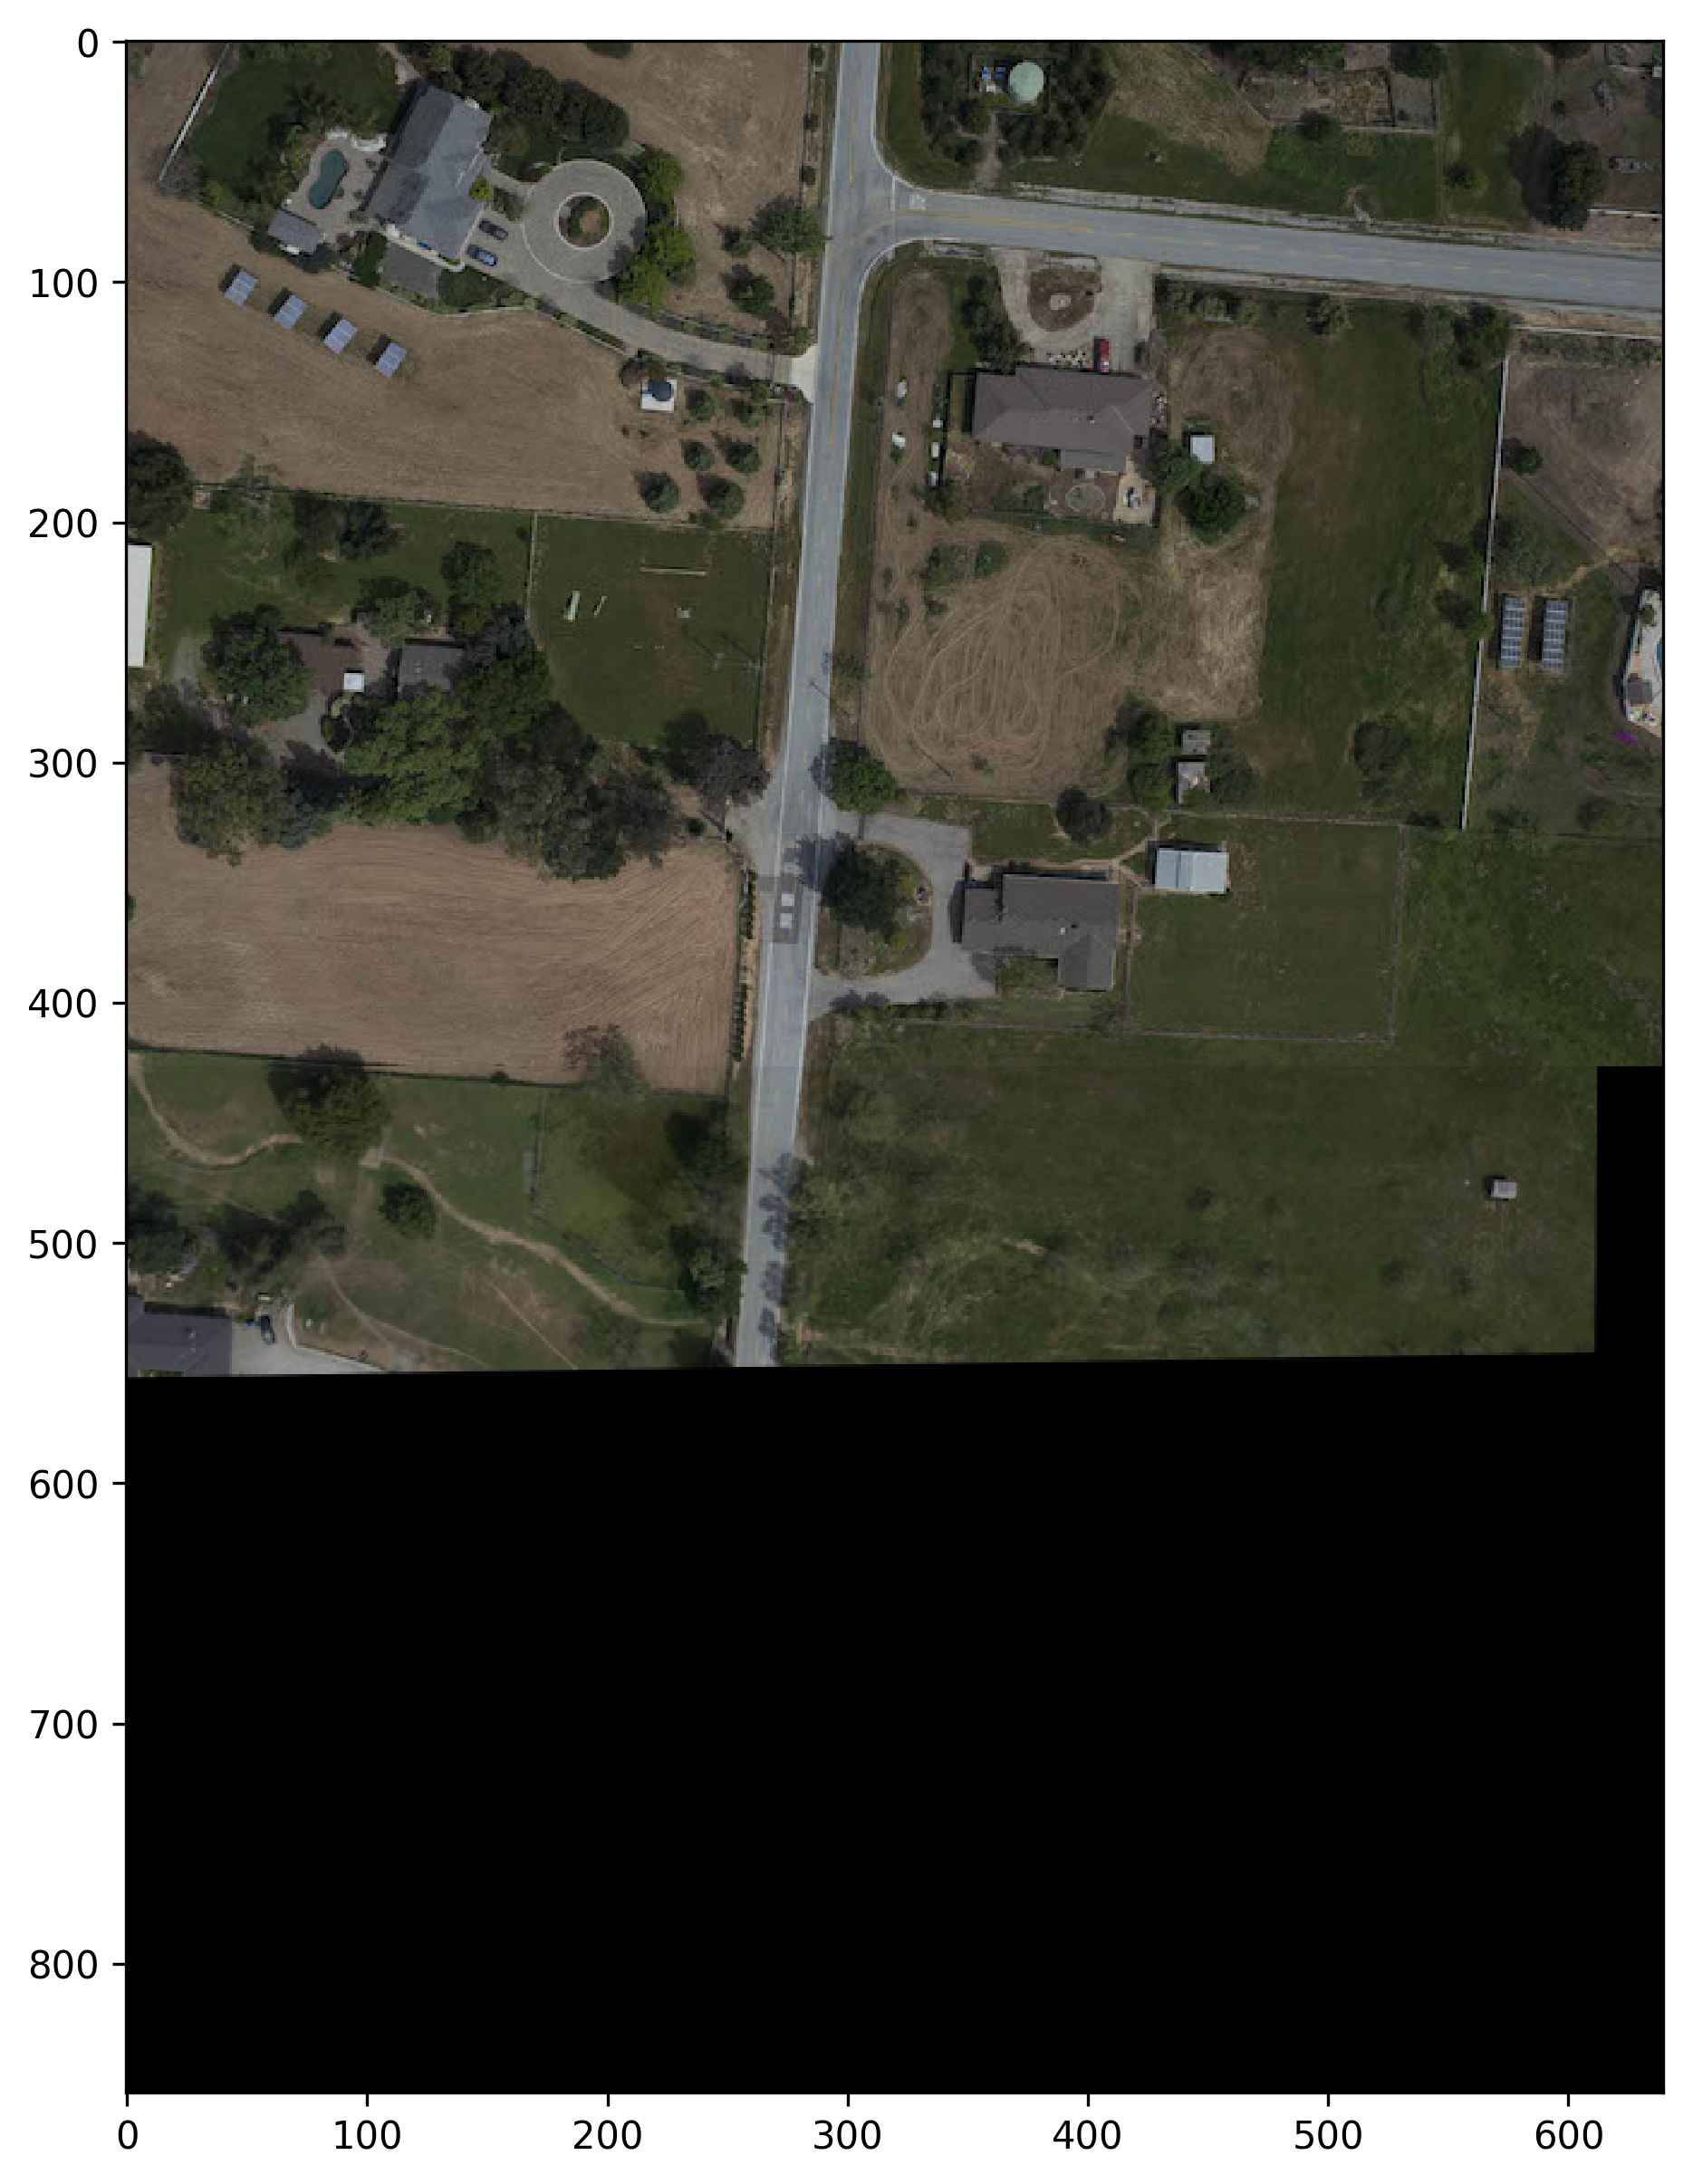
\includegraphics[width=0.99\textwidth]{pics/vertical_panorama_img_3}
	\caption{. \label{fig:pan-img-3}}   
\end{center} 
\end{figure}

\begin{figure*}
\begin{center}
	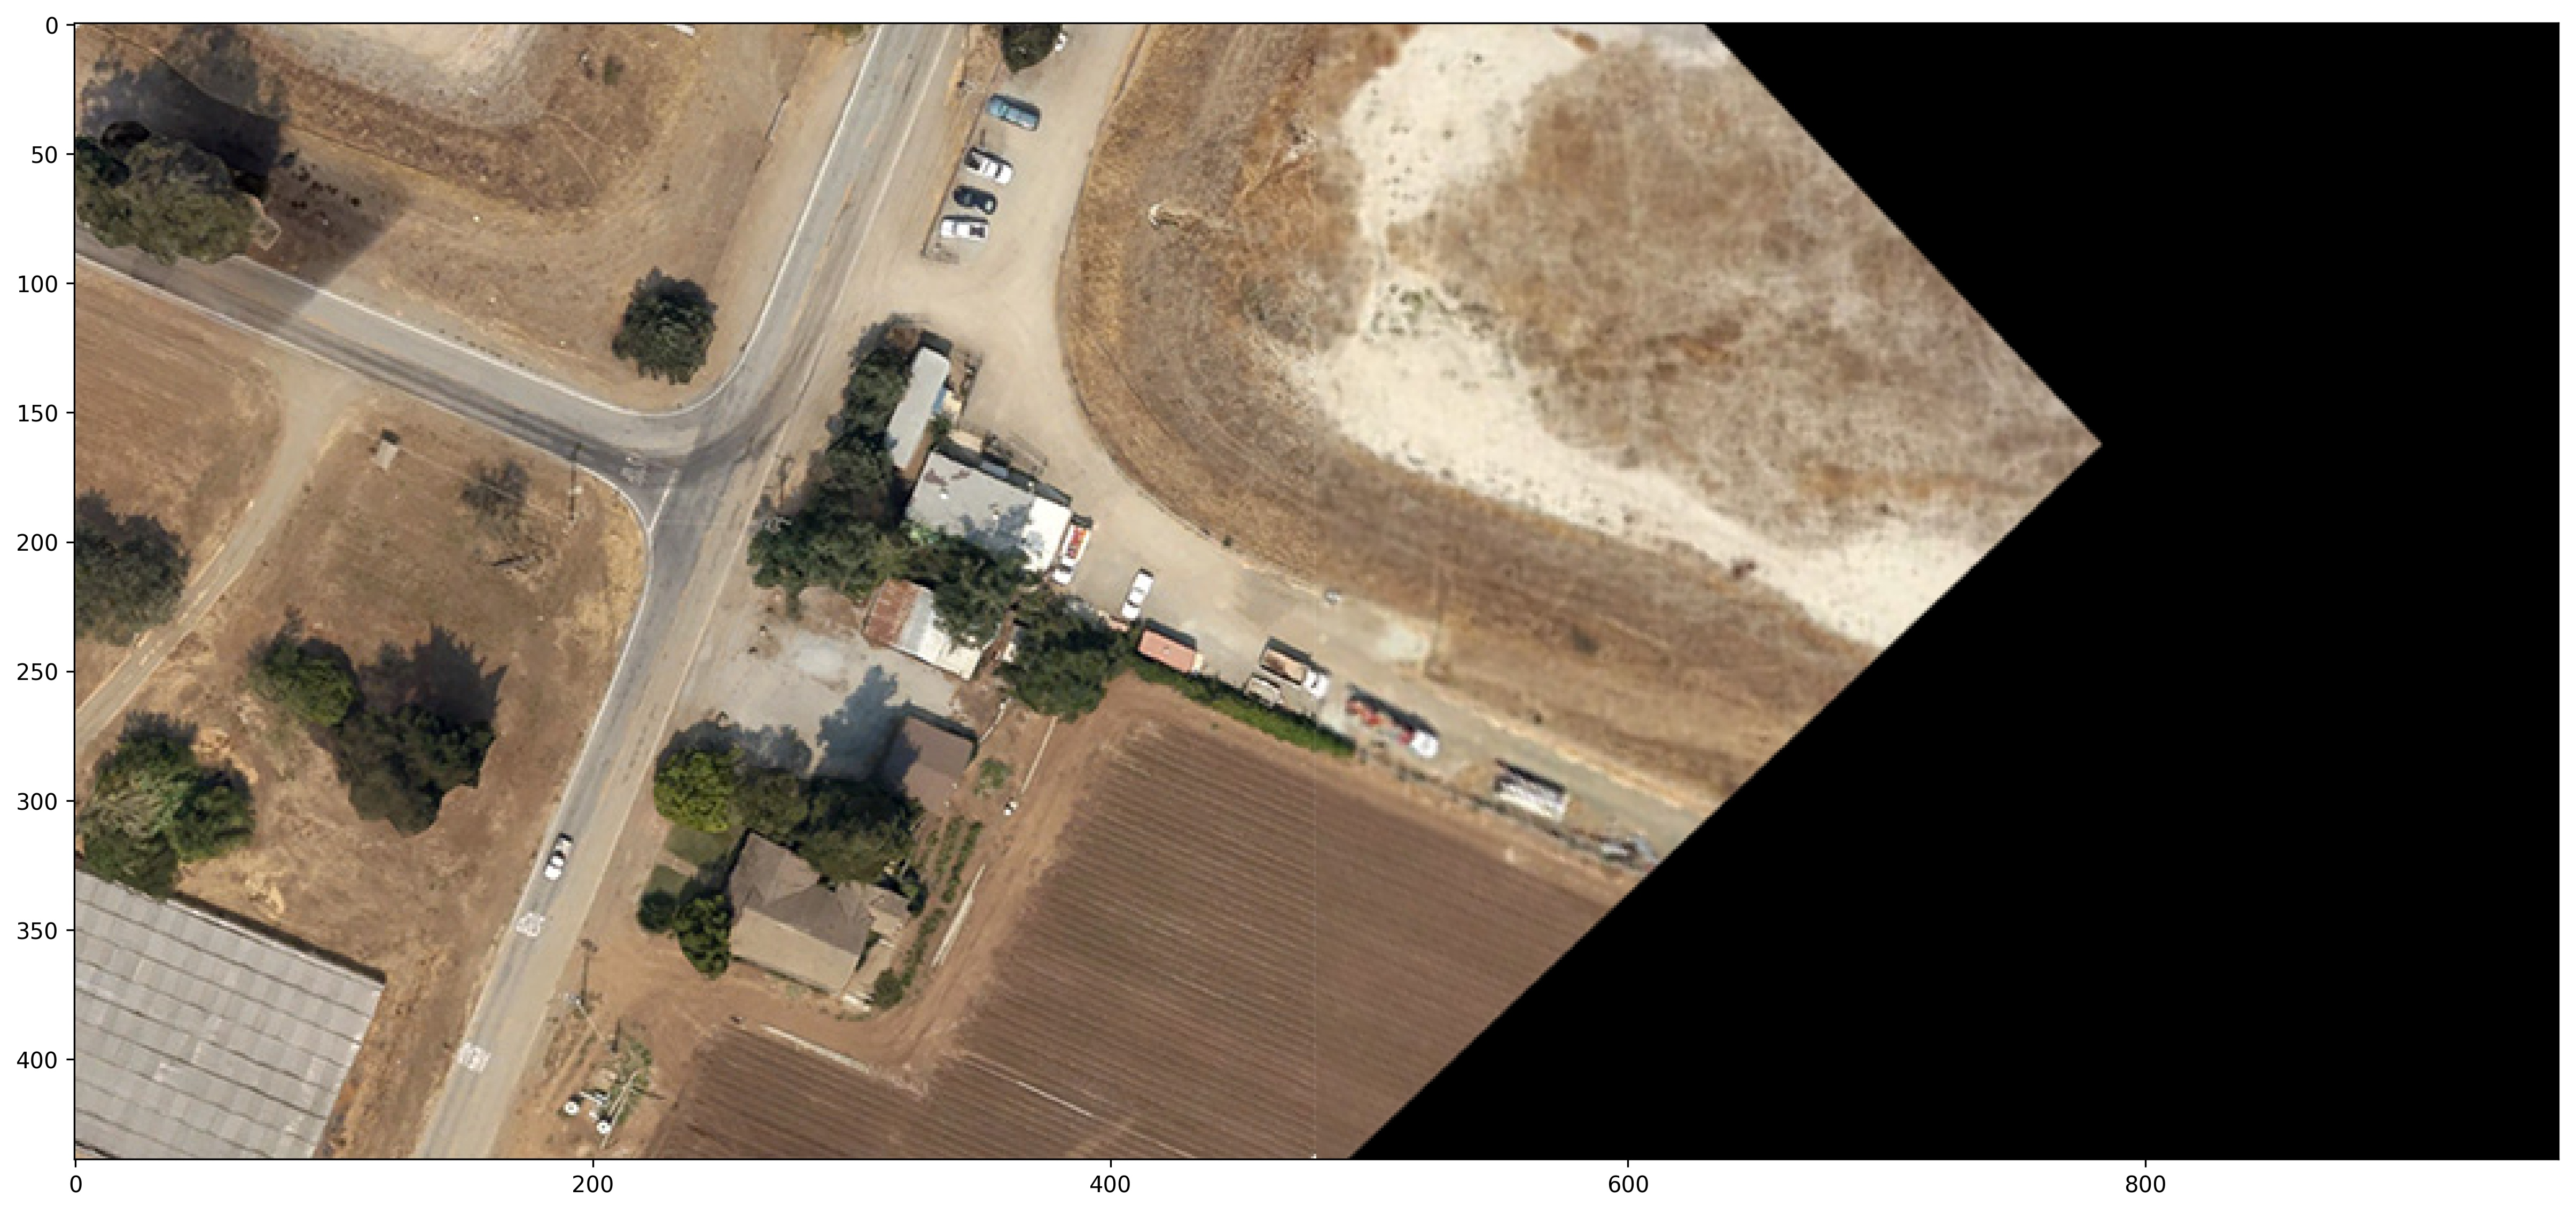
\includegraphics[width=0.99\textwidth]{pics/horizontal_panorama_img_4}
	\caption{. \label{fig:pan-img-4}}   
\end{center} 
\end{figure*}

%\CITEONE{Silva}{Silva_2010} for papers with one author.
%\CITETWO{Silva}{Souza}{Silva_2010b} for papers with two authors.
%\CITEN{Silva}{Silva_2010c} for papers with three or more authors.

%%% Add section %%%%%%%%%%%%%%%%%%%%%%%%%%%%%%%%%%%%%%%%%%%%%%%%%%%%%%%%%%%%%%%%%%
\section{Conclusion}

...

%%% References %%%%%%%%%%%%%%%%%%%%%%%%%%%%%%%%%%%%%%%%%%%%%%%%%%%%%%%%%%%%%%%%%%%
{\small
\bibliographystyle{unsrt}
\bibliography{refs}
}


\end{document}